%\section{Scénario d'utilisation}
\chapter{Scénario d'utilisation}
\markboth{\MakeUppercase{Scénario d'utilisation}}{}     

	\section{Aspect général}

		\paragraph{Le plateau :}
			L'affichage du plateau prend la majorité de la fenêtre.
			Les entités sont représentées par des lettres dans des cases de la couleur de leur équipe.
			Les \^{} sur fond gris sont les montagnes.
			Les cases possédant une bordure pointillée noire permettent d'identifier les forts et arsenaux.
			Les cases vertes représentent les possibilités de mouvement	de l'entité sélectionnée (l'infanterie bleu sur la figure~\ref{fig:affichage_zone_influence}). 
			Notons que l'unité ne peut pas se déplacer sur une case déja occupée.
			Lorsqu'une entité risque d'être détruite au prochain tour, son symbole est entouré de ( ).
			Lorsqu'elle est forcée de se retirer au prochain tour, son symbole est entouré de [ ].
	
		\paragraph{Le menu :}
	
			Le menu contient différents éléments :
			\begin{itemize}
			\item[-]Le bouton de chargement en haut permet de charger une situation depuis un fichier
			\item[-]Les checkboxes permettent d'activer ou de désactiver les communications
			\item[-]Les grands boutons permettent de changer le mode d'affichage
			\end{itemize}

	\section{Les modes d'affichage}

		Ne pouvant pas afficher la totalité des informations sur le plateau, (unités, potentiels, zones dangereuses, points faibles) nous
		avons décidé de créer plusieurs modes d'affichage distincts afin de ne pas le surcharger.

		\subsection{Mode unités}
			\begin{figure}[!h]
				\centerline{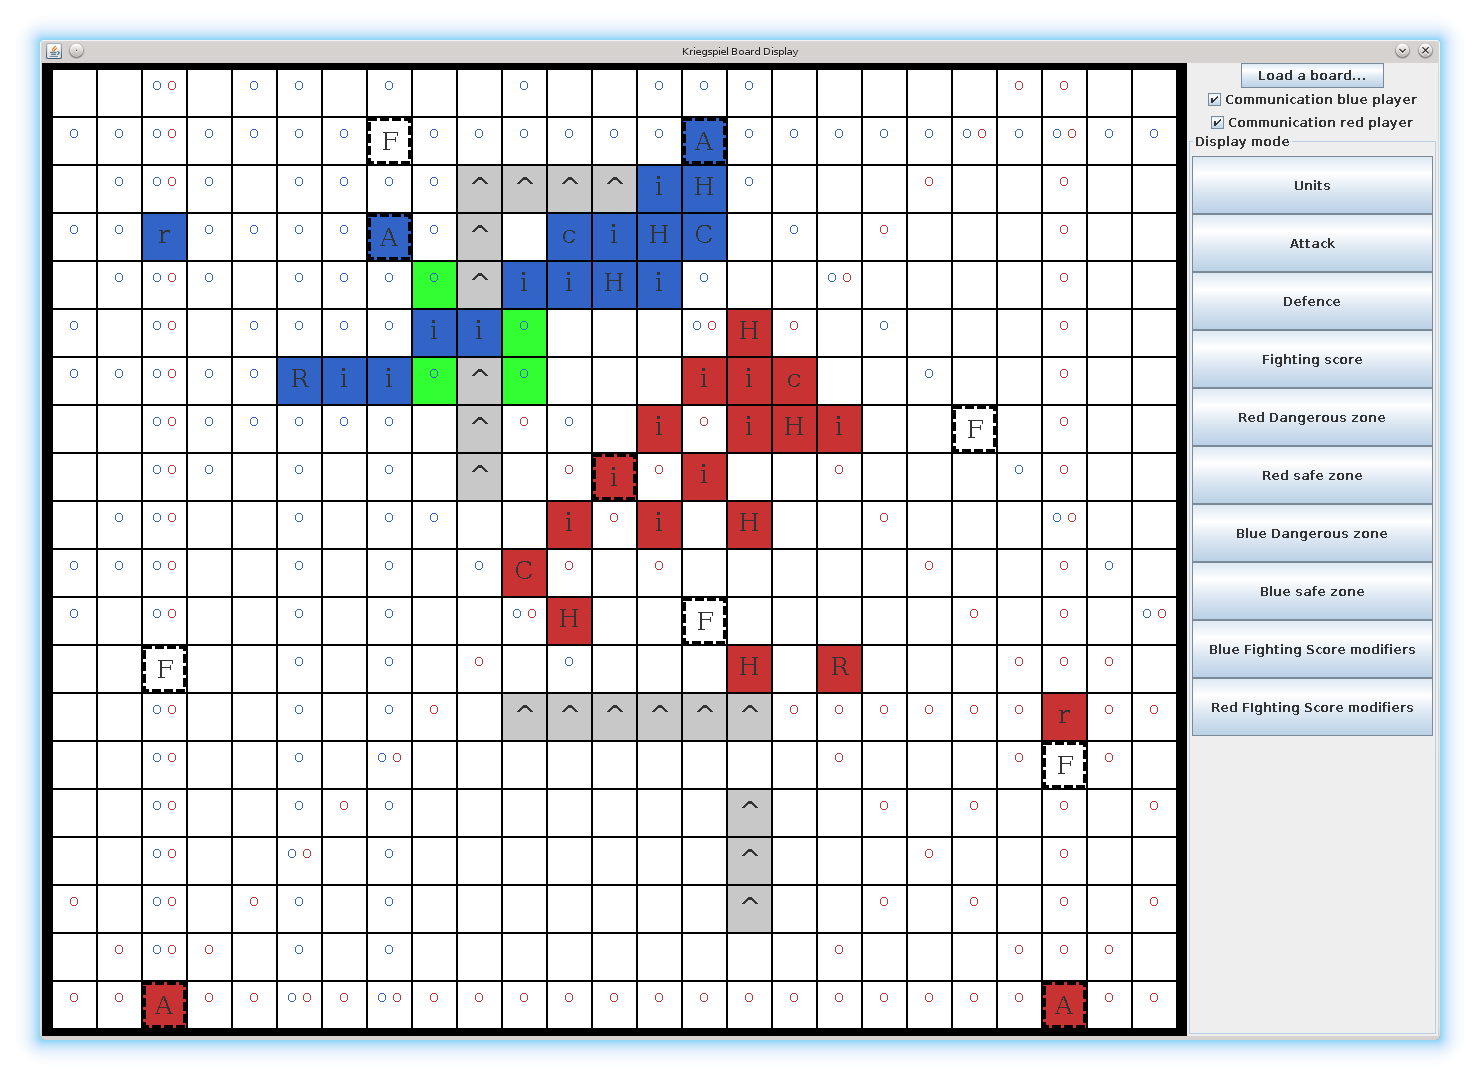
\includegraphics[scale=0.4]{images/screen_units.png}}
				\caption{Exemple d'affichage du mode unités}
				\label{fig:mode_unite}
			\end{figure}

			C'est le mode d'affichage principal, les symboles des unités sont affichés dans les cases.
			\clearpage

		\subsection{Modes attaque/défense}

			\begin{figure}[!h]
				\centerline{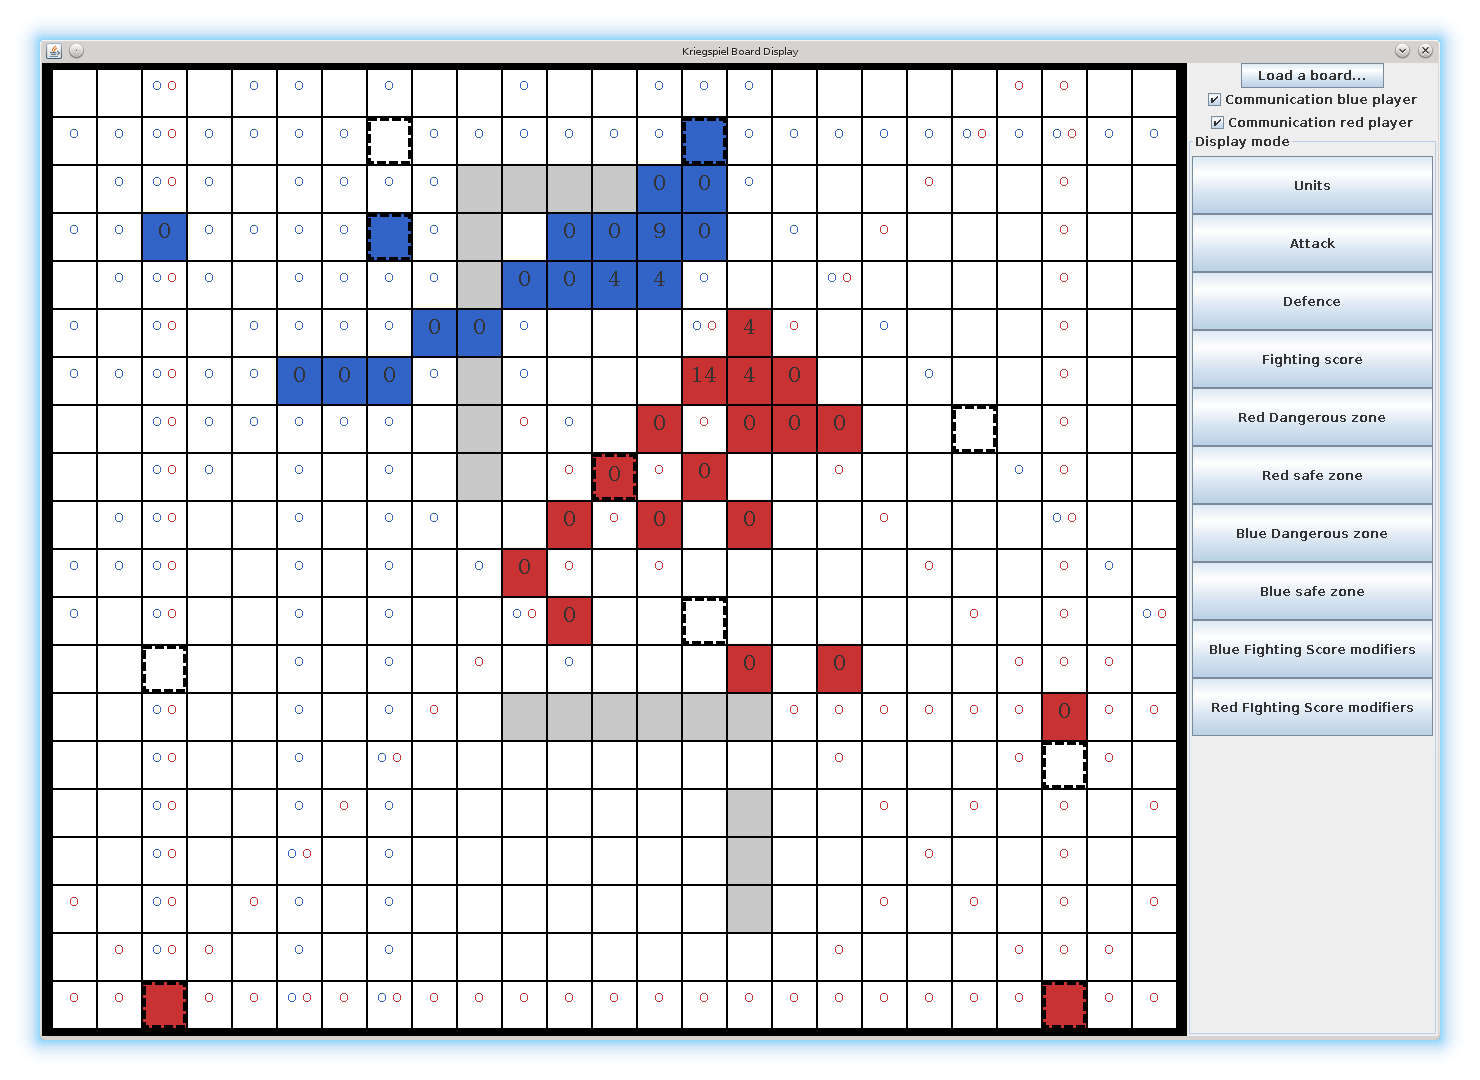
\includegraphics[scale=0.4]{images/screen_def.png}}
				\caption{Exemple d'affichage du mode attaque}
			\end{figure}

			Dans le mode attaque, le total d'attaque potentielle subie est affiché à la place du symbole de chaque unité.
			Dans le mode défense, le total de défense de l'unité est affiché.
			Ces valeurs sont calculées à partir des indications données dans les règles du jeu.
			\clearpage	

		\subsection{Mode score de combat / points faibles}

			\begin{figure}[!h]
				\centerline{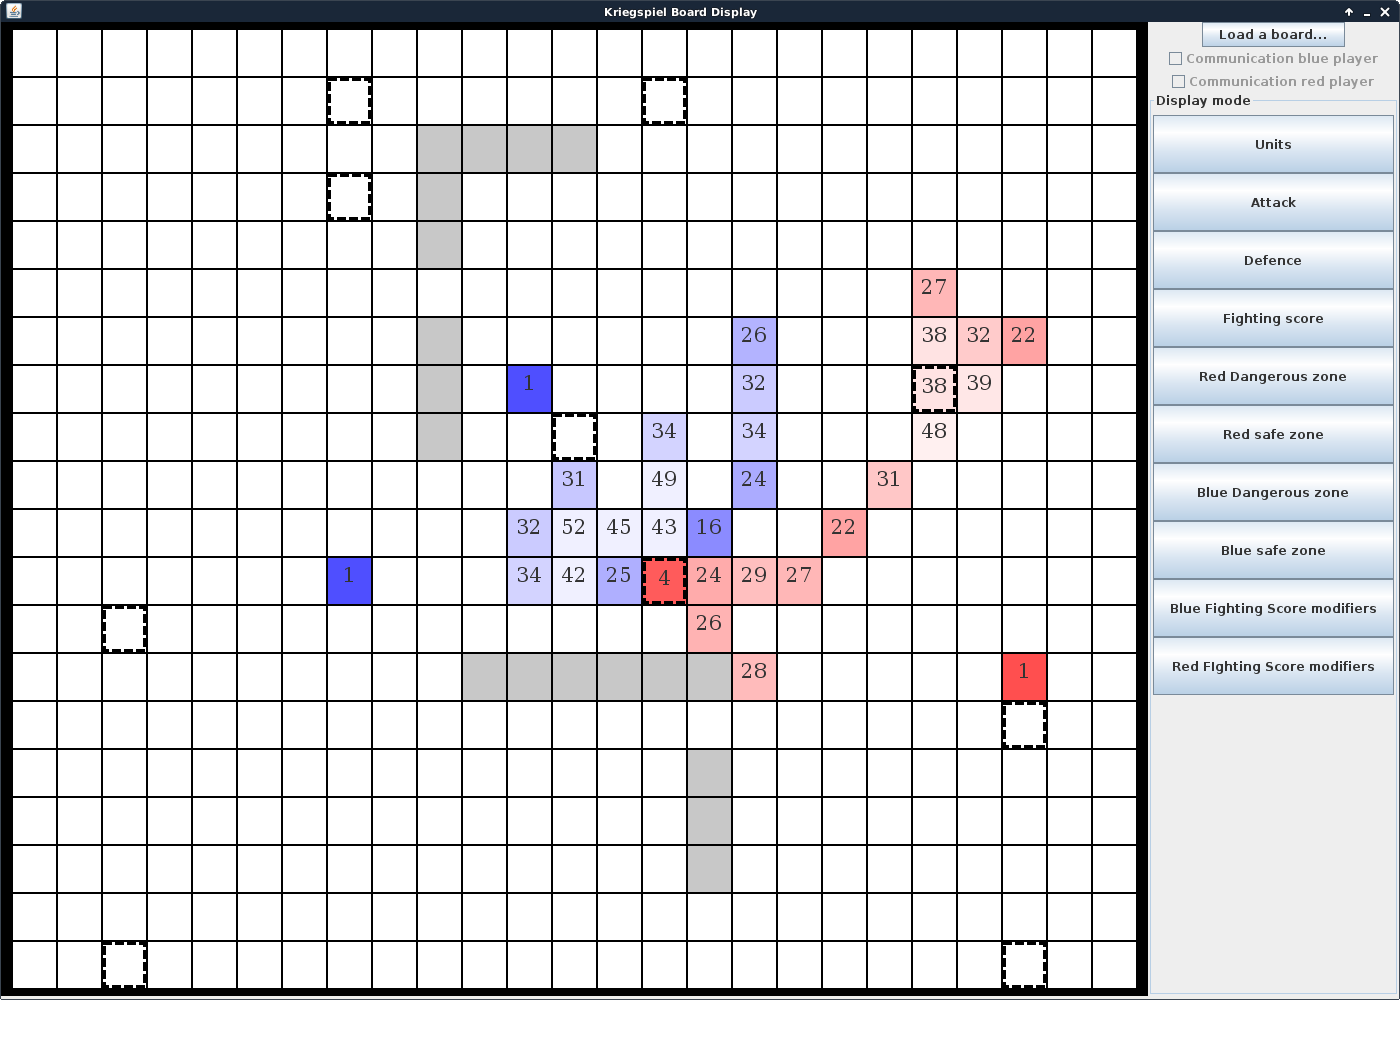
\includegraphics[scale=0.35]{images/screen_fscore.png}}
				\caption{Le mode score de combat appliqué a une situation du livre}
				\label{fig:partie_livre}
			\end{figure}
			
			\paragraph{}
			Le mode score de combat permet de voir les unités en situation de force ou de faiblesse.
			Plus l'unité est foncée, plus son score est faible et donc plus elle est vulnérable.
            Les scores affichés dans les cases sont le résultat de la soustraction de l'attaque subit par l'unité à son score de défence. Cela signifie que si ce score est négatif, l'unité peut être détruite (voir les règles) et la case sera mise en évidence par une couleur plus foncée.
			Cette matrice permet donc de déterminer les points faibles d'une armée s'ils existent.
			
			\paragraph{}
			Pour vérifier l'utilité de cette matrice, nous avons transcrit une situation de jeu commentée du livre de Debord \cite{ref2} (partie retranscrite
			par la figure~\ref{fig:partie_livre}). Nous avons ensuite lu les commentaires à propos de cette partie voir si la stratégie utilisée concordait bien
			avec les points faibles indiqués par notre matrice.

			\epigraph{La figure 6 représente deux armées groupées, sur le point d'engager la bataille, après avoir marché l'une et l'autre pour s'assurer certaines positions
			de départ. Le camp Nord est à pied d'oeuvre pour prendre d'assaut la forteresse en L15 qui constitue le pivot de manoeuvre du camp Sud.}{--- \textup{Guy Debord}, Le Jeu de la Guerre - Page 159}
						
			\paragraph{}
			Il est clair d'après la partie commentée que le fort est le point clef de cette bataille, or nous pouvons remarquer que la matrice des points faibles
			met justement en exergue l'unité se trouvant sur le fort. Il s'agit donc d'une situation pour laquelle cette matrice pourra être parfaitement exploitable
			pour une éventuelle future prise de décision.	
			
			\clearpage	

		\subsection{Modes zone sûre/zone dangereuse}
			\begin{figure}[!h]
				\centerline{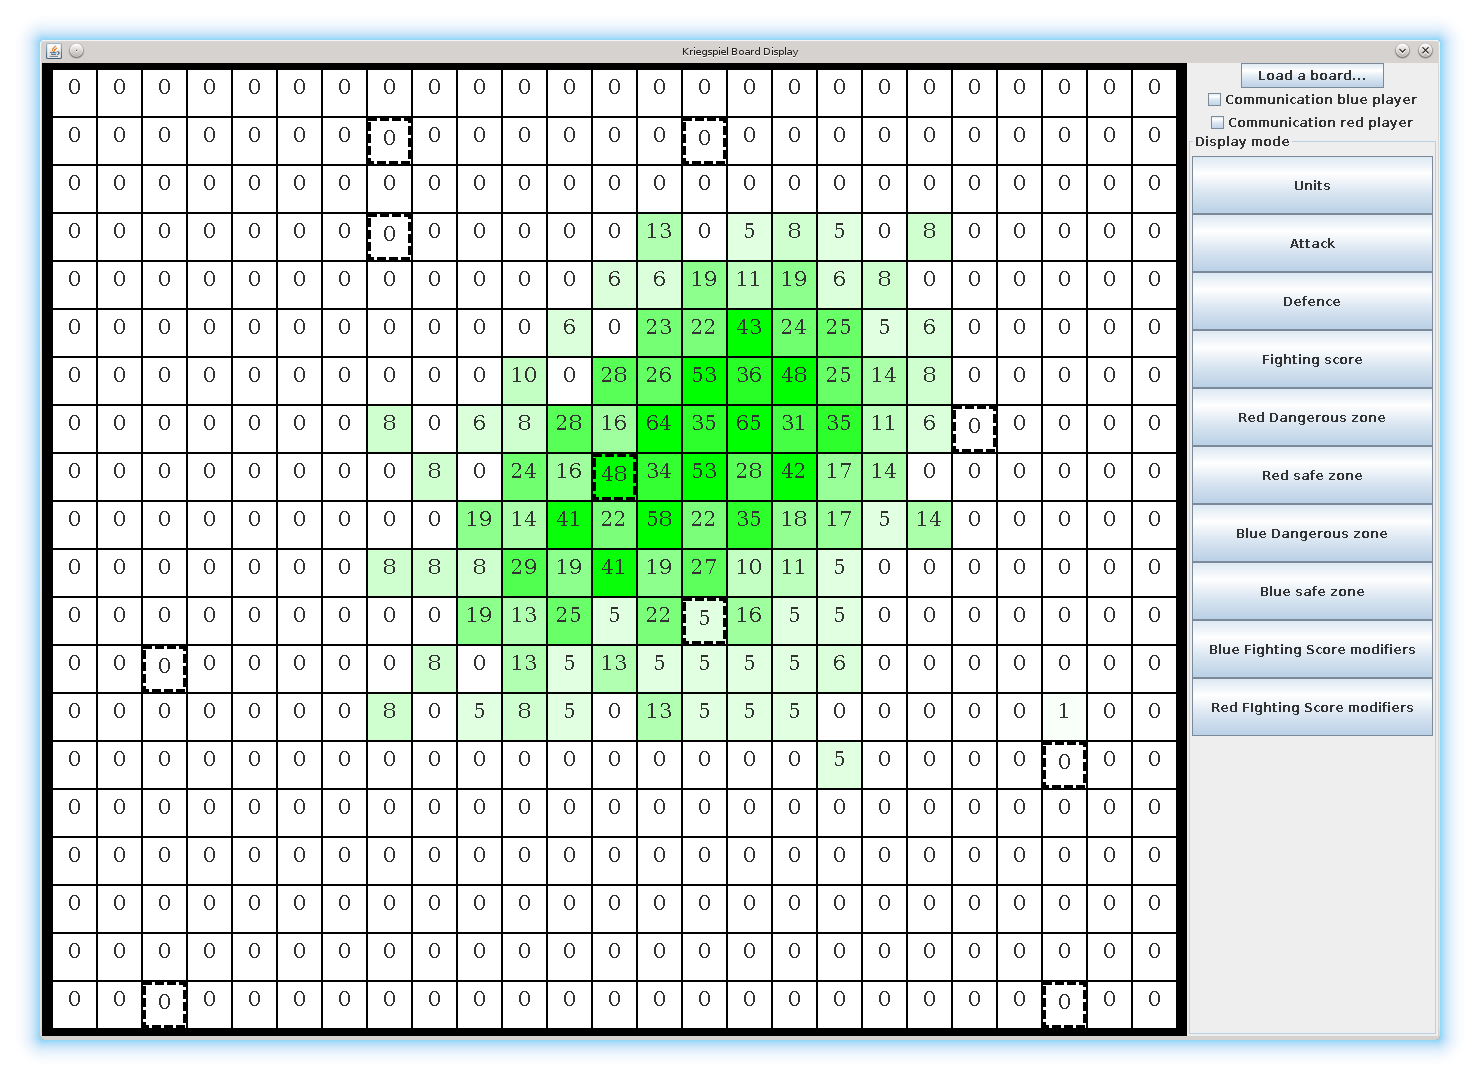
\includegraphics[scale=0.4]{images/screen_safe.png}}
				\caption{Exemple d'affichage du mode zone sûre}
			\end{figure}

			Dans le mode zone sûre, la matrice de défense de l'équipe choisie est affichée.
			Dans le mode zone dangereuse, la matrice d'attaque de l'équipe choisie est affichée
			Plus les cases sont foncées, plus elles sont sûres (respectivement dangereuses) pour l'équipe.
			Ici c'est la zone sûre de l'équipe rouge qui est affichée.
            Dans le cas de la matrice de défence, les scores affichés dans chaque case indiquent le score de défense octroyé par les unités alliés (dans le cas où il serait décidé d'y placer une unité, elle bénéficierait du score de défence affiché dans la case, en plus de sa propre défence).
            Dans le cas de la matrice d'attaque, les scores affichés dans chaque case indiquent le score d'attaque subit des unités adverses (une unité placée sur une de ces cases subira donc le score d'attaque qui y est affiché).

			\clearpage

		\subsection{Modes modificateur de score de combat}
			\begin{figure}[!h]
				\centerline{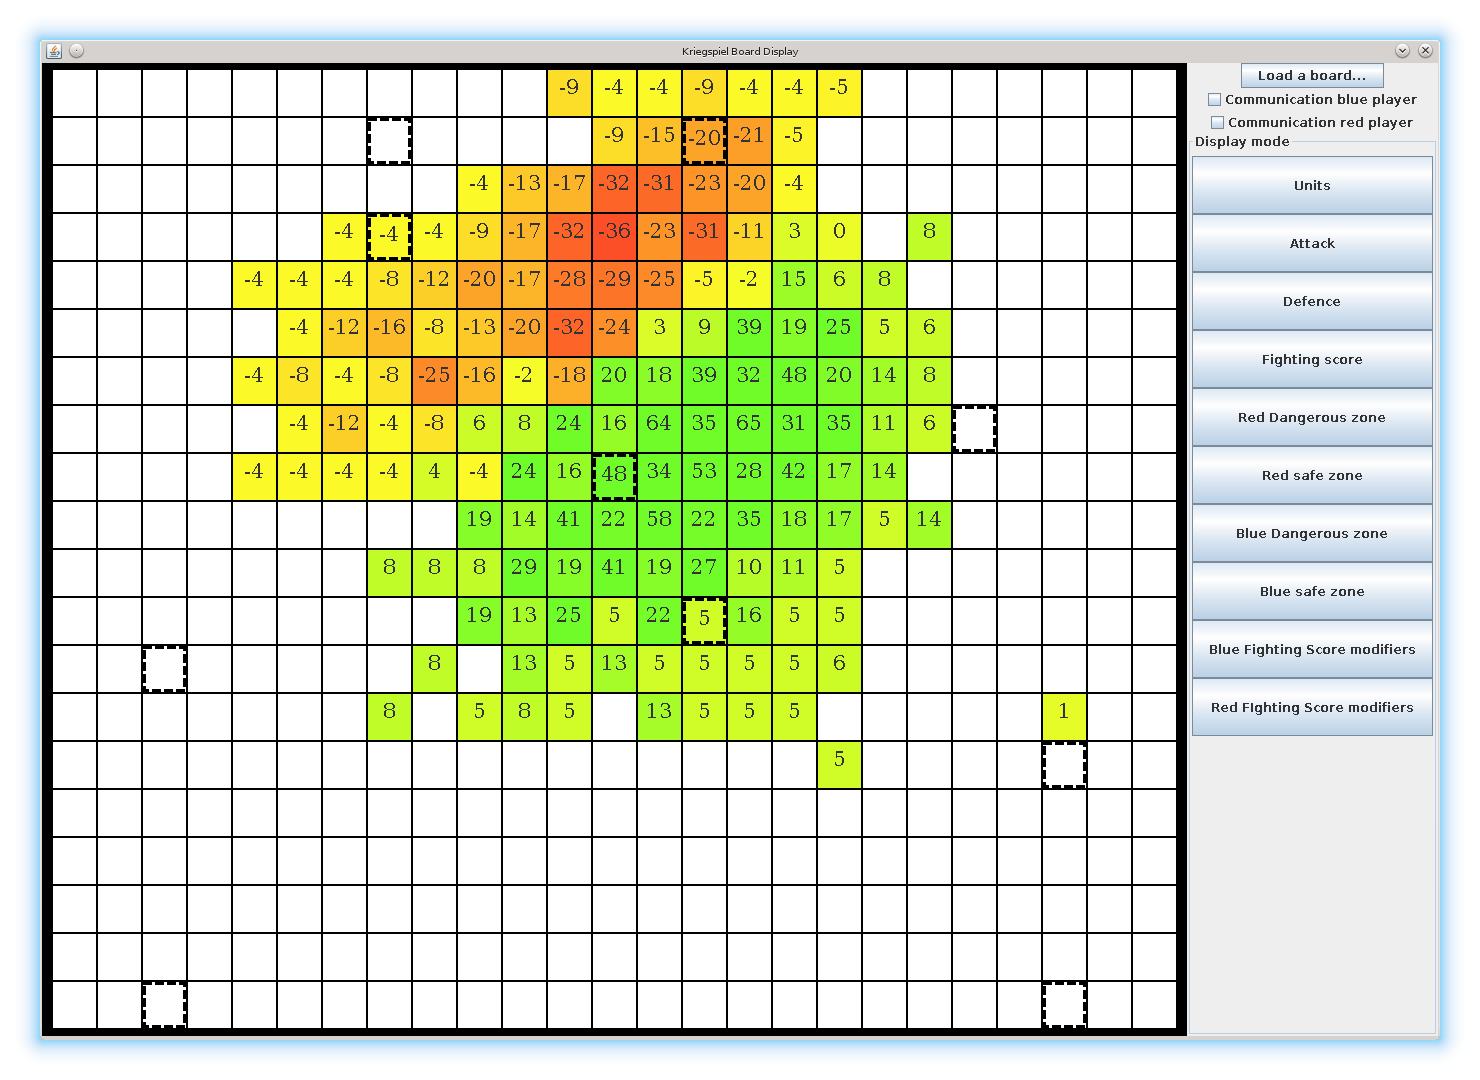
\includegraphics[scale=0.4]{images/screen_fsmod.png}}
				\caption{Exemple d'affichage du mode modificateur du score de combat}
			\end{figure}
			Dans ces derniers modes d'affichage, on utilise les zones sûres et dangereuses pour calculer pour chaque cas le modificateur
			qui serait appliqué au score de combat d'une unité si elle y était présente.
			Dans ce cas, on peut par exemple voir qu'une unité de l'équipe rouge se plaçant sur le fort au milieu recevrait un bonus de 48 a son score de combat, la rendant très difficile a détruire.

	\section{Autres fonctionnalités}

		\subsection{Lignes de communication}

			\begin{figure}[!h]
			\centerline{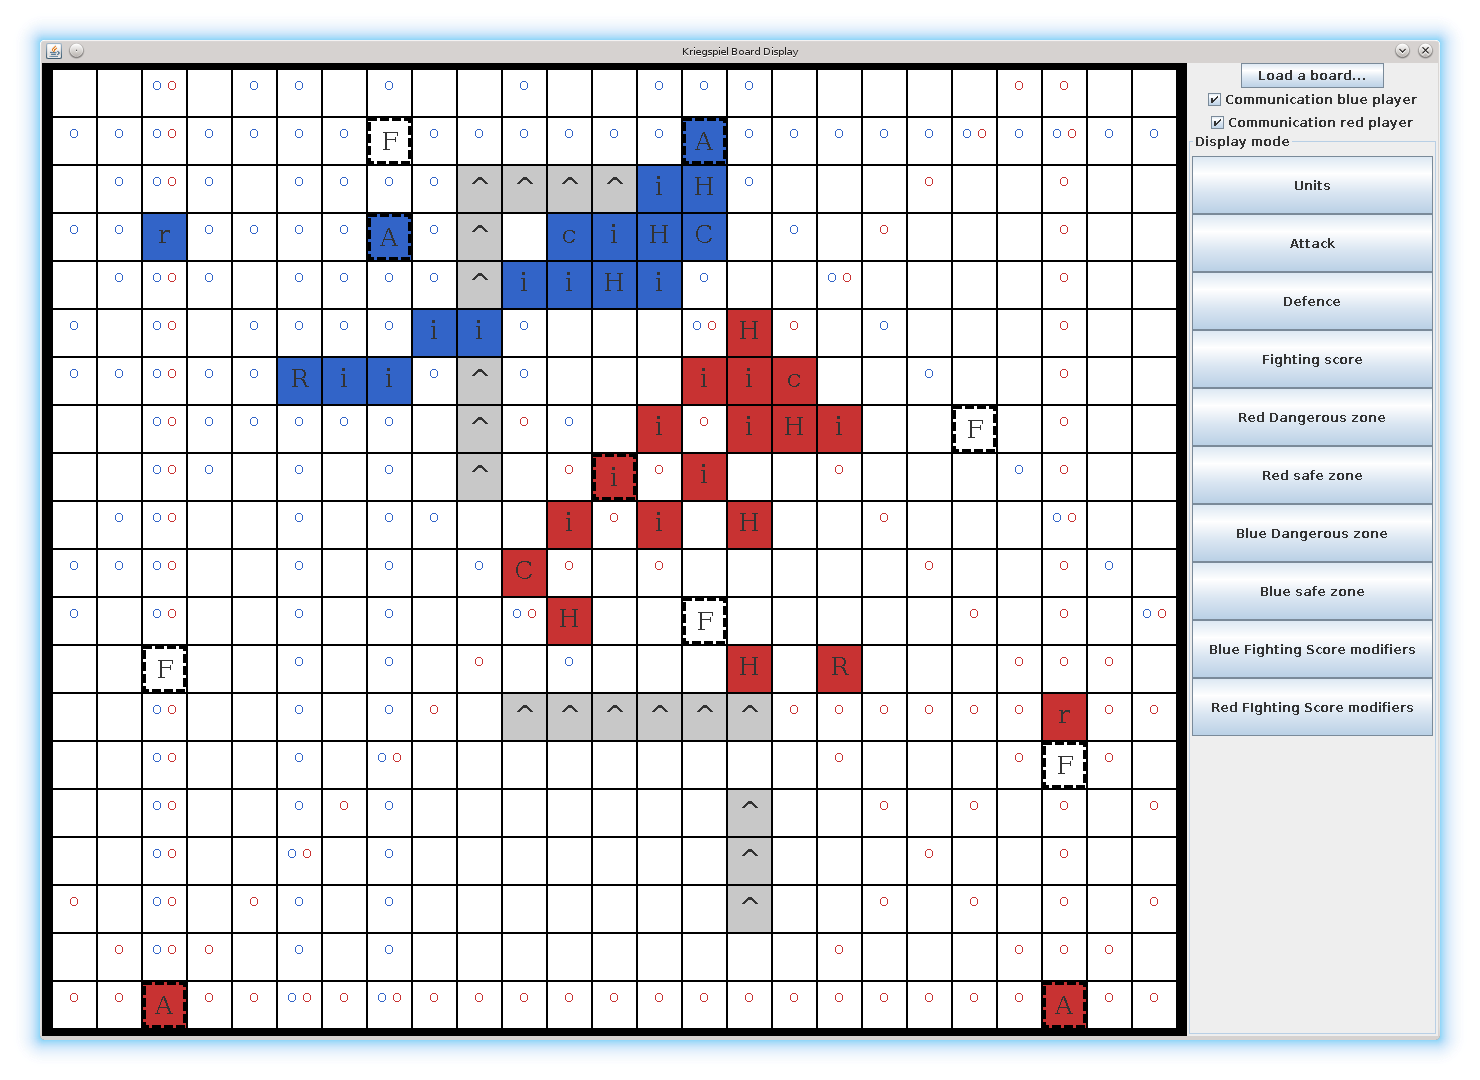
\includegraphics[scale=0.35]{images/screen_com.png}}
			\caption{Exemple d'affichage des lignes de communication}
			\end{figure}
			Les lignes de communication sont représentées par des cercles de la couleur de l'équipe sur les cases vides.
			Les unités déconnectées ont une teinte plus claire que les unités connectées.
			On peut remarquer que les unités adverses (excepté les relais) bloquent les communications et que les relais alliés les propagent. 
			(sauf relais ne se trouvant pas sur une ligne de communication)
			
			\clearpage

		\subsection{Raccourcis clavier}
			Avant d'implémenter le menu, nous avions mis en place des racourcis clavier afin de modifier rapidement les options d'affichage.
			Ces raccourcis ont été maintenus et fonctionnent correctement de concert avec les boutons mais nous avons cessé d'en rajouter 
			en considérant qu'il était inutile d'apprendre des raccourcis alors qu'un clic sur un bouton est aussi rapide et efficace.
			Il est donc possible d'afficher / cacher les lignes de communications avec les touches 0 et 1 (pour les équipes 0 et 1) du pavé numérique.
			Il est également possible de changer de mode d'affichage entre Unités (u) Attaque (a) et Défense (d).
